\section{Results}

Firstly, we verify that the algorithm works. We can do this by comparing to the original serial implementation. From comparing different iteration numbers, it was observed that for small trees, these are exactly the same, however, for bigger ones, some tiny differences in pixels start showing due to some floating point differences, which are barely visible even when the images are shown side by side as in Figure \ref{fig:comparison}.
	
\begin{figure}
	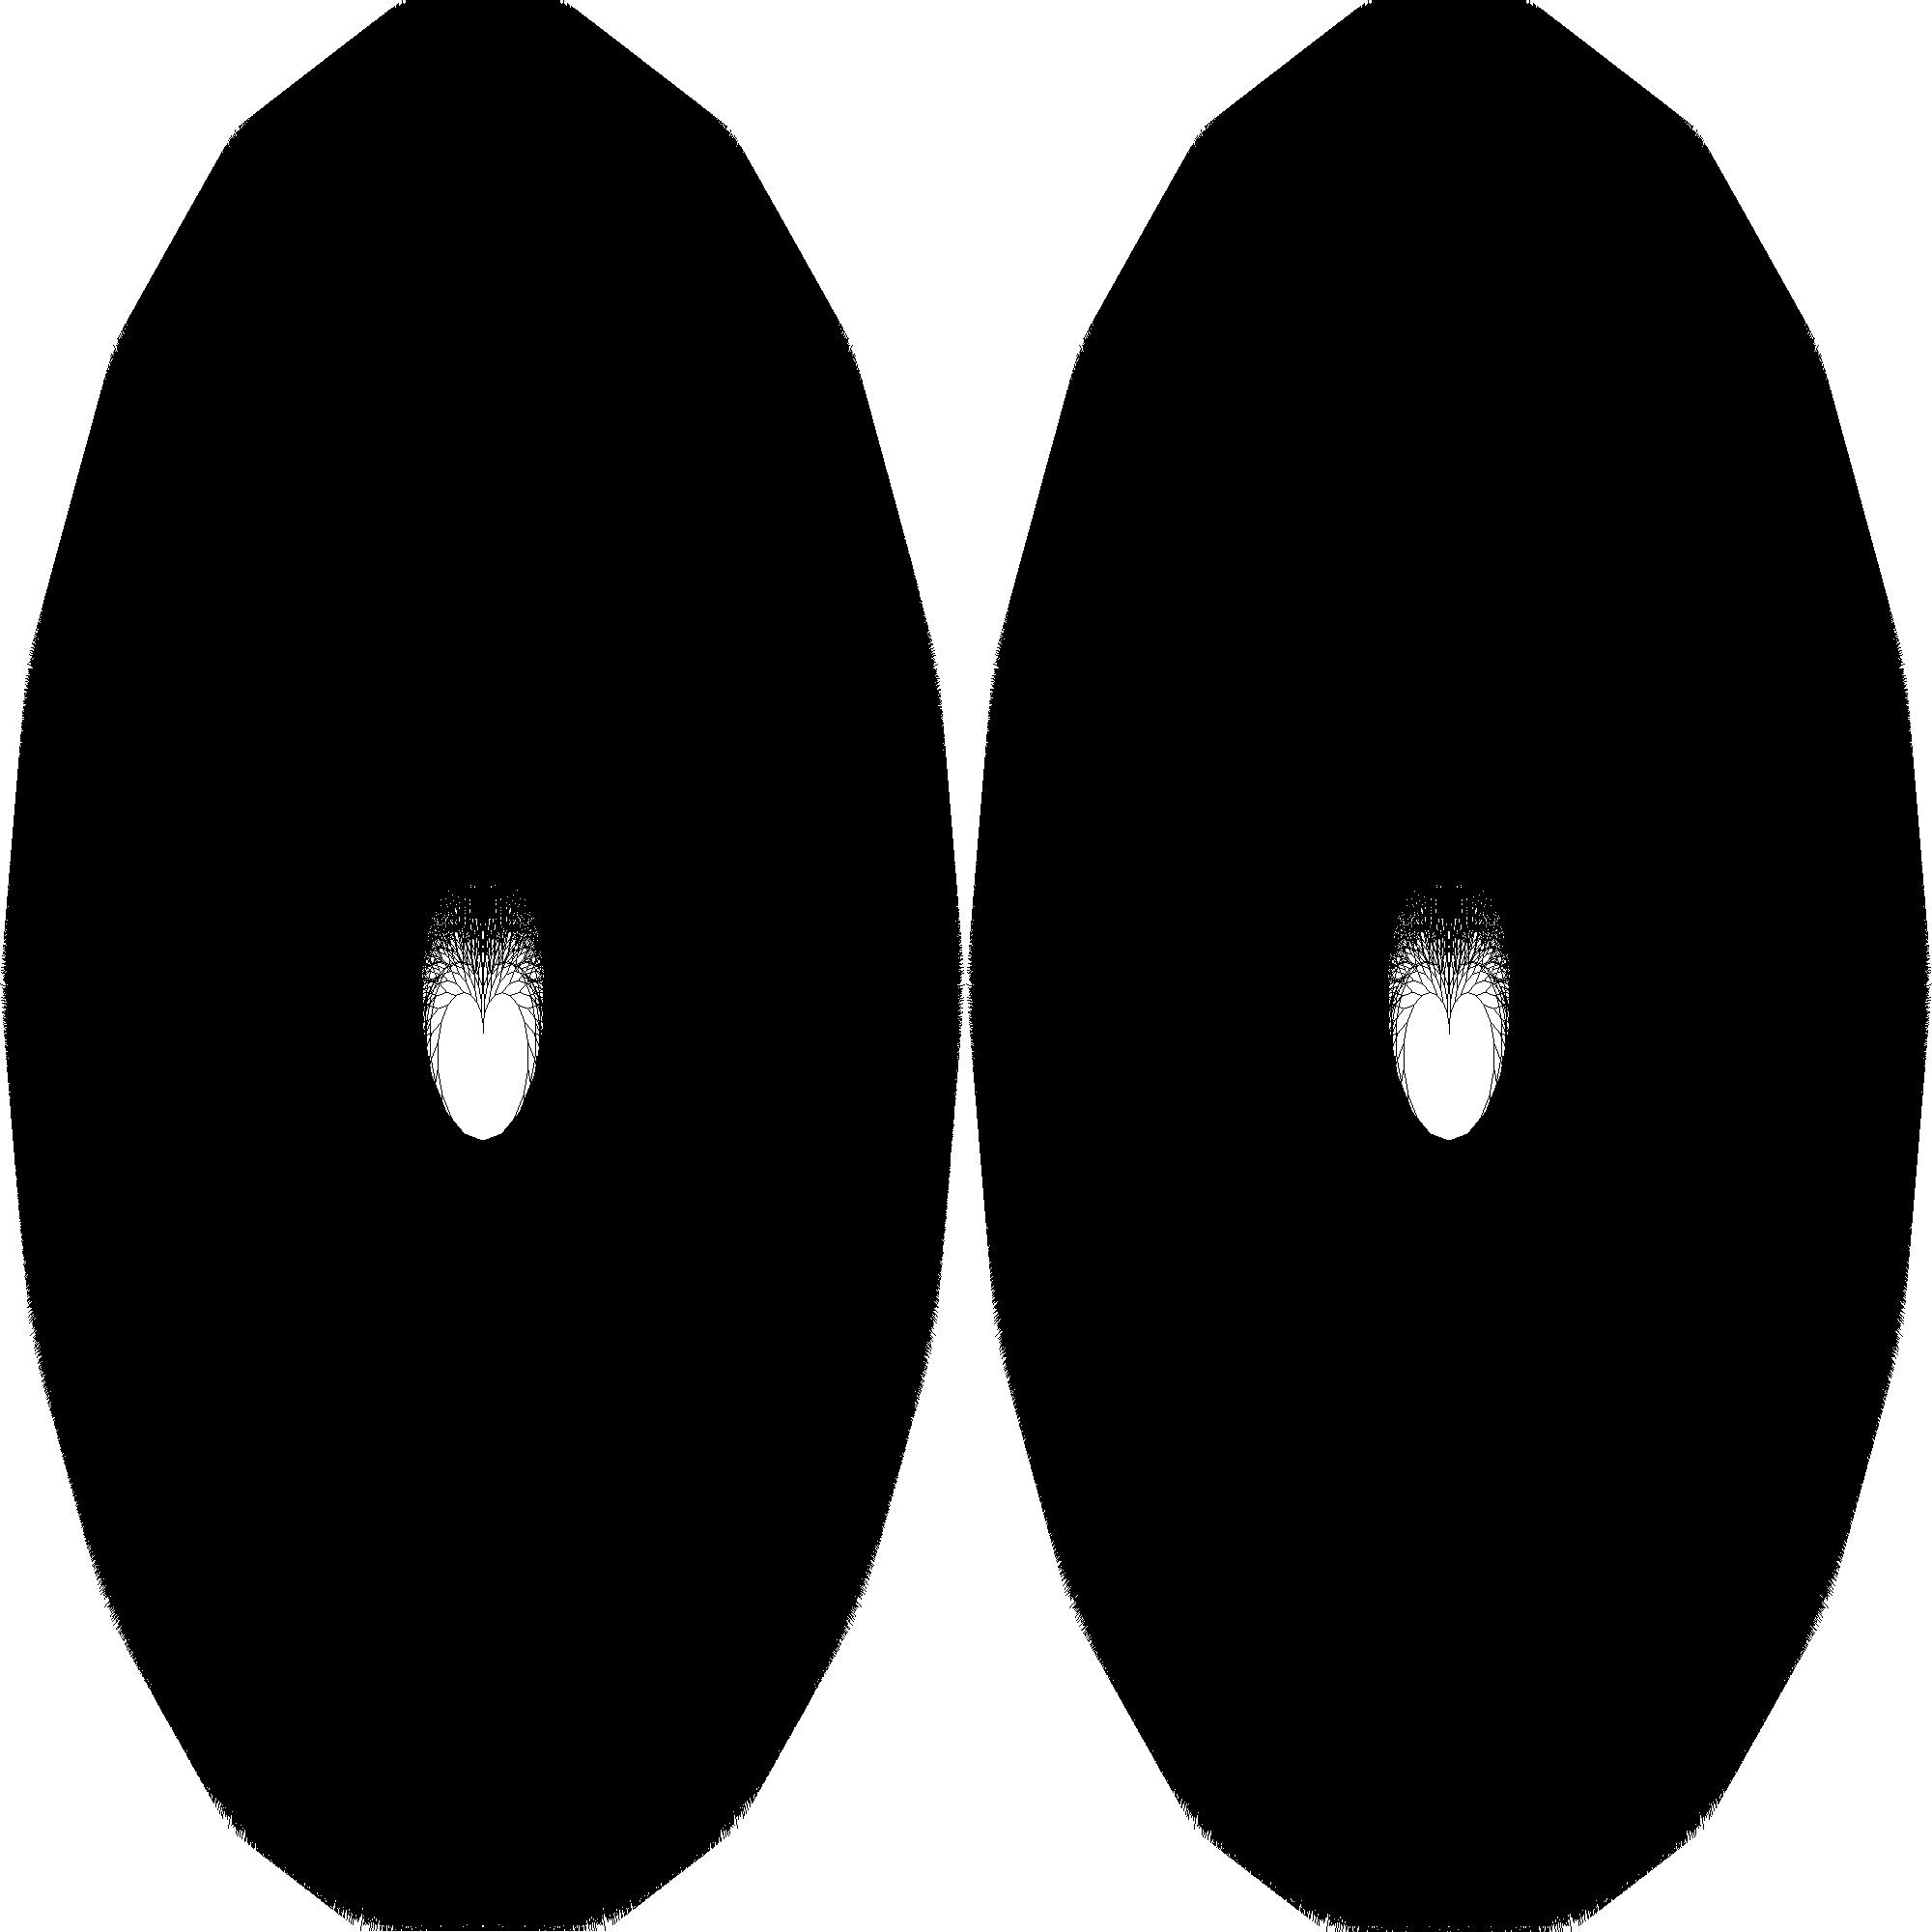
\includegraphics[width=.95\linewidth]{Images/comparison.png}
	\centering
	\caption{Two fractals generated by the program, left by the serial version and right by the parallel version. The following were the parameters used: WxH=1000x2000 m=1.1 $\theta$=20 n=25}
	\label{fig:comparison}
\end{figure}

Next we compare the speed it takes for the two parts when they are run serially on the CPU against in parallel on the GPU. The graph in figure \ref{fig:timing} compares the two when we vary n. For small values, the serial implementation is slightly faster, however, as we pass a certain threshold, we see that the parallel implementation scales up orders of magnitudes better.


\begin{figure*}
	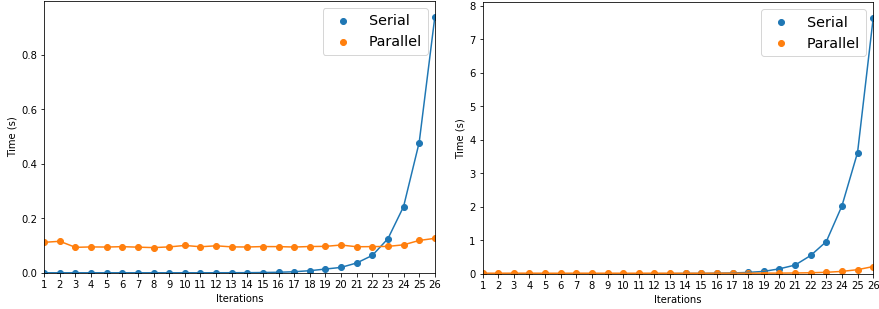
\includegraphics[width=.95\linewidth]{Images/timing.png}
	\centering
	\caption{The timing results for generating the points (left) and synthesizing the image (right) when WxH=500x500 m=1 $\theta$=90 and n is varying}
	\label{fig:timing}
\end{figure*}

With regards to further optimization on the parallel side, it was found to be difficult to optimise further. When the sine and cosine maps were added to shared memory, this did not make a noticeable difference in performance. We also avoid warp divergence as much as possible given the problem. Memory management is also being taken care of properly, by only using items in the host and devices when they are needed in the respective device, freeing memory as soon when it is no longer in use and avoiding unnecessary data transfers. These optimizations are reflected in the obtained performance results as we obtain a noticeable speed-up.

When the profiler timeline was observed (Appendix A) it was determined that most of the time taken is to draw the points. This time increases even further if we increase the image size.

If we compare the rough theoretic speed to the practical speed for part 1, lets say that we do this for 26 iterations, in the theoretic we get 1053948 ClockCycles, which, given each processor works at 980MHz, this should theoretically take 0.001075 seconds, however ends up taking 0.12647 seconds. This is most likely due to the needs of synchronization, and having to make multiple kernel calls, not to mention memory allocation.